\section{Data}\label{sec:data}

\subsection{Registry crawl}
We seed a breadth-first crawl of the npm registry with the \NSeeds{} packages that have the most
dependents, as listed in \pkg{npm-high-impact} (version~1.13.0). For every package the crawl fetches the
latest-version manifest from \url{https://registry.npmjs.org} and extracts:
\begin{itemize}
  \item the four dependency tables (production, optional, peer and development) with their raw version
        constraints;
  \item the presence of \pkg{preinstall}, \pkg{install} or \pkg{postinstall} scripts, or npm's
        \pkg{hasInstallScript} flag;
  \item build provenance, from the \pkg{dist.attestations} field;
  \item the list of maintainer accounts.
\end{itemize}
The crawl follows installed dependency types (production, optional, peer) up to a node budget. It does
not follow development dependencies, which consumers do not install. Ecosystem-wide dependent counts
come from the deps.dev API.

We classify every constraint by how permissive it is to automatic updates, following node-semver
semantics:
\begin{itemize}
  \item \emph{exact} (\texttt{1.2.3}), \emph{tilde} (\texttt{\~{}1.2.3}), \emph{caret}
        (\texttt{\^{}1.2.3}) or \emph{wildcard} (\texttt{*}, dist-tags, open upper bounds);
  \item caret ranges on \texttt{0.x} behave like tilde, and \texttt{\^{}0.0.x} like exact;
  \item for \texttt{||} unions the loosest branch wins;
  \item \texttt{npm:} aliases resolve to their target;
  \item git, file and URL specifiers are \emph{non-registry} and are dropped, since registry publishes
        cannot reach them.
\end{itemize}

We build three graphs from the same seed list:
\begin{itemize}
  \item a \FiveN-package sample;
  \item the \MainN-package \emph{main} graph;
  \item the \emph{full closure}, in which the crawl ran out of new packages at \FullRaw{} packages.
\end{itemize}
Edges to packages outside a sample are dropped.

\paragraph{Spam-ring cleaning.}
The full closure contained a complete 25-package clique of mutually dependent packages with
fruit-pair names, all owned by one maintainer. It belongs to a farm of \SpamRemoved{} reward-farming
packages that entered the crawl through a single dependent. On its own this clique set
$\lambda_{\max}=24$. We therefore drop every strongly connected component with at least 10 packages and
edge density at least $0.5$, together with the other packages of maintainers who own most of such a
ring. Legitimate monorepo cycles survive this filter because they are far sparser, for example
\pkg{@stdlib} (density 0.26), \pkg{@yarnpkg} (0.13) and \pkg{@eggjs} (0.10).

\subsection{Synthetic benchmark}
As a controlled baseline we generate directed scale-free graphs with the Bollob\'as--Borgs--Chayes--Riordan
model, using \pkg{networkx}'s \pkg{scale\_free\_graph} with $n=\SynN$ and a narrowed out-degree. Because
node index equals creation order, we orient every edge from newer to older packages. This removes a
large artificial cycle among hubs that the raw generator creates, which real npm does not have. SemVer
types, install scripts, provenance and maintainers are assigned at empirical rates. Maintainer
portfolios follow a Zipf-like distribution.

\subsection{Structure of the main graph}
\Cref{tab:data} summarises the graphs. The main graph has \MainN{} packages and \MainE{} dependency
edges. Its SemVer mix is \MainSemverCaret{} caret, \MainSemverExact{} exact, \MainSemverTilde{} tilde and
\MainSemverWildcard{} wildcard. Only \MainHooks{} of packages declare install scripts, while
\MainProvenance{} publish with provenance.

The graph is close to a DAG. It has \MainNontrivialSCC{} non-trivial strongly connected components, the
largest of which has \MainLargestSCC{} packages. The spectral radius of the weighted contagion matrix is
$\lambda_{\max}=\MainLambdaW$, which sets the mean-field threshold $\tau_c=1/\lambda_{\max}=\MainTauTheory$.
This value is determined by a single dense \pkg{@stdlib} cluster rather than by the ecosystem as a
whole.

The maximum blast radius, i.e.\ the largest number of transitive dependents of any package, is
\MainMaxReach{}, and the mean is \MainMeanReach. Out-degree (direct dependents) is heavy-tailed
(\cref{fig:degree}). A discrete power-law fit gives $\alpha=\MainAlphaOut$ for $k\geq\MainXminOut$, but
a likelihood-ratio test prefers a lognormal (normalized log-likelihood ratio $\MainLLRLognormalOut$,
$p=\MainPLognormalOut$). This agrees with the finding that strictly scale-free real networks are
rare~\citep{broido2019rare}. Degree assortativity is weakly negative ($r_{\text{out,in}}=\MainAssortOutIn$).

\begin{table}[t]
\centering
\caption{The graphs used in this study. Blast radius is the number of transitive dependents. The
synthetic graph is a DAG by construction, so its $\lambda_{\max}=0$ and $\tau_c=\infty$.}
\label{tab:data}
\begin{tabular}{lrrrrrr}
\toprule
Graph & Packages & Edges & Largest SCC & $\lambda_{\max}(W)$ & $\tau_c$ & Max.\ blast radius \\
\midrule
npm 5k & \FiveN & \FiveE & \FiveLargestSCC & \FiveLambdaW & \FiveTauTheory & \FiveMaxReach \\
npm 10k (main) & \MainN & \MainE & \MainLargestSCC & \MainLambdaW & \MainTauTheory & \MainMaxReach \\
npm full closure & \FullN & \FullE & \FullLargestSCC & \FullLambdaW & \FullTauTheory & \FullMaxReach \\
Synthetic & \SynN & \SynE & \SynLargestSCC & \SynLambdaW & \SynTauTheory & \SynMaxReach \\
\bottomrule
\end{tabular}
\end{table}

\begin{figure}[t]
\centering
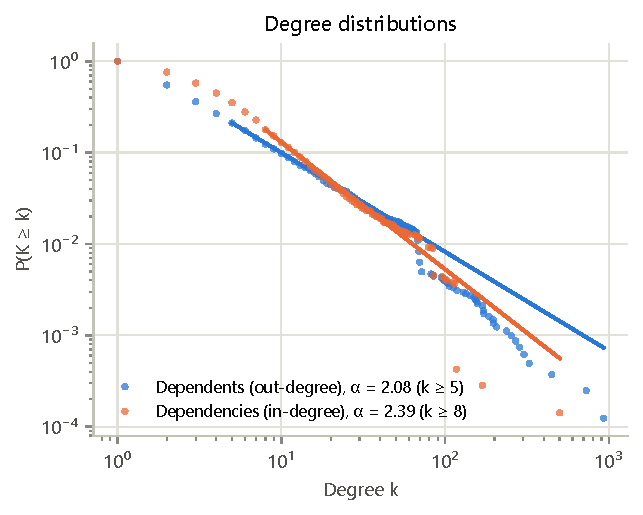
\includegraphics[width=0.55\linewidth]{fig1_degree_distribution.pdf}
\caption{Complementary cumulative degree distributions of the main graph, with discrete power-law fits
above $x_{\min}$. Dependents correspond to the contagion out-degree.}
\label{fig:degree}
\end{figure}
